
\documentclass{beamer}
\usepackage[latin1]{inputenc}
%\usetheme{Montpellier}
%\usetheme{Boadilla}
%\usecolortheme[RGB={204,51,255}]{structure}
%\usecolortheme[named=purple]{structure}
%\usecolortheme[RGB={62,128,62}]{structure}
\usecolortheme[RGB={62,62,128}]{structure}
%\definecolor{reddish}{rgb}{0.3,0.15,0.3}
%\definecolor{light}{rgb}{0.8,0.6,0.8}
%\definecolor{reddish}{rgb}{.5,0.15,0.15}
\definecolor{reddish}{rgb}{0.5,0.3,0.4}
%\definecolor{light}{rgb}{0.8,0.6,0.8}
\definecolor{reddish}{rgb}{.7,0.25,0.25}
\definecolor{greenish}{rgb}{.25,0.8,0.25}
\definecolor{blueish}{rgb}{.25,0.25,0.7}
\definecolor{purple}{rgb}{.5,0.0,0.5}
\usepackage{graphicx}
\usepackage{pstricks}
\usepackage{epsfig}
\newcommand{\btVFill}{\vskip0pt plus 1filll}

\setbeamertemplate{navigation symbols}{}

\newcommand{\crish}{\color{reddish}}
\newcommand{\cgish}{\color{greenish}}
\newcommand{\cbla}{\color{black}}
\newcommand{\cred}{\color{red}}
\newcommand{\cblu}{\color{blue}}
\newcommand{\cgrish}{\color{green}}

\newcommand{\sm}{\color{reddish}$}
\newcommand{\fm}{$\color{black}{}}

\newcommand{\letter}[1]{\color{blue}\texttt{#1}\color{black}}
 \newcommand{\binary}[1]{\color{red}\texttt{#1}\color{black}}

\usepackage{tikz}
\usetikzlibrary{arrows,decorations.markings,positioning}
\usepackage{epstopdf}
\usetikzlibrary{fit}
\usepackage{pgfplots}

\title[The Bayesian Brain lecture 3]{The Kalman filter: the Bayesian Brain lecture 2}
\author{COMSM0075 Information Processing and Brain}
\institute{\texttt{comsm0075.github.io}}
\date{October 2020}

\begin{document}

\maketitle


\pgfmathdeclarefunction{gauss}{2}{%
  \pgfmathparse{1/(#2*sqrt(2*pi))*exp(-((x-#1)^2)/(2*#2^2))}%
}

\begin{frame}{Kalman filter}
  \begin{quote}
The Kalman filter uses Bayesian fusion to estimate location based on noisy measurement and on dead reckoning.
  \end{quote}

\end{frame}

\begin{frame}{The problem}
\begin{center}
\includegraphics[width=6cm]{cyclist1.png}
\end{center}
\end{frame}


\begin{frame}{Dead reckoning}
\begin{center}
\includegraphics[width=6cm]{cyclist2.png}
\end{center}
\end{frame}


\begin{frame}{Measurement}
\begin{center}
\includegraphics[width=6cm]{cyclist_gps.png}
\end{center}
\end{frame}


\begin{frame}{Two sources of position}
\begin{center}
\includegraphics[width=6cm]{cyclist_gps1.png}
\end{center}
\end{frame}


\begin{frame}{Two sources of position}
\begin{center}
\includegraphics[width=6cm]{cyclist_gps2.png}
\end{center}
\end{frame}


\begin{frame}{Everything is Gau\ss{}ian}
1) specified by the mean and variance: \cblu$\mu=4$\cbla{} and \cblu$\sigma^2=1$\cbla{}
  \vskip 1cm
\begin{tikzpicture}
  \begin{axis}[
  no markers, domain=0:8, samples=100,
  axis lines*=left, xlabel=$x$, ylabel=$y$,
  every axis y label/.style={at=(current axis.above origin),anchor=south},
  every axis x label/.style={at=(current axis.right of origin),anchor=west},
  height=5cm, width=12cm,
  xtick={4}, ytick=\empty,
  xtick=\empty,
  ytick=\empty,
  enlargelimits=false, clip=false, axis on top,
  grid = major
  ]
  \addplot [very thick,blue] {gauss(4,1)};
\end{axis}
  \draw (8.25,2.2) node{\color{blue}$p(x)\sim \mathcal{N}(\mu,\sigma^2)$\cbla};
\end{tikzpicture}
\end{frame}


\begin{frame}{Everything is Gau\ss{}ian}
2) start with Gau\ss{}ians and stay with Gau\ss{}ians.
  \vskip 1cm
  \begin{tikzpicture}
  \begin{axis}[
  no markers, domain=0:8, samples=100,
  axis lines*=left, xlabel=$x$, ylabel=$y$,
  every axis y label/.style={at=(current axis.above origin),anchor=south},
  every axis x label/.style={at=(current axis.right of origin),anchor=west},
  height=5cm, width=12cm,
  xtick={4}, ytick=\empty,
  xtick=\empty,
  ytick=\empty,
  enlargelimits=false, clip=false, axis on top,
  grid = major
    ]
    \addplot [very thick,blue] {gauss(4,1)};
    \addplot [very thick,red] {gauss(2,2)};
    \addplot [very thick,black] {gauss(3.56,0.9)};
\end{axis}
\end{tikzpicture}
\end{frame}

\begin{frame}{Some equations}
  \crish$$
  \mathbf{\bar{x}}=\left(\begin{array}{c}\bar{s}\\\bar{v}\end{array}\right)
  $$\cbla{}
  \flushleft{represents the current estimates of the position and
  speed: or more precisely they are the means of our probability
  distributions representing our belief about the position and speed.}
\end{frame}

\begin{frame}{Covariance}
\crish$$
P_{ij}=\langle (x_i-\bar{x}_i)(x_j-\bar{x}_j)\rangle
$$\cbla{}
\flushleft{The idea is to update both the mean and the covariance; which is
equivalent for Gau\ss{}ian distributions to updating the distribution.}
\end{frame}

\begin{frame}{Dead reckoning}
The position and speed is given by \crish$\mathbf{x}$\cbla{} which is drawn from a Gau\ss{}ian with mean \crish$\mathbf{\bar{x}}$\cbla{} with covariance \crish$P$\cbla{}. Without noise
  \crish$$
  x\rightarrow x_a = x+v\delta t
  $$\cbla{}
  \flushleft{We are assuming the speed is constant; it is easy to include intentional changes of speed by including a \textbf{control vector}; we don't do that here.}
  \crish$$
  v\rightarrow v
  $$\cbla{}
\end{frame}


\begin{frame}{Dead reckoning}
\crish$$
\mathbf{x}_a=F\mathbf{x}+\mathbf{w}
$$\cbla{}
\flushleft{where \crish$F$\cbla{} is the motion matrix}
\crish$$
F=\left(\begin{array}{cc}1&\delta t\\0&1\end{array}\right)
$$\cbla{} and \crish$\mathbf{w}$\cbla{} is zero mean Gau\ss{}ian noise
  with covariance matrix \crish$Q$\cbla{} .
\end{frame}

\begin{frame}{Dead reckoning}
  \crish$$
\mathbf{x}_a=F\mathbf{x}+\mathbf{w}
$$\cbla{}
\flushleft{Now take the average:}
\crish$$
\mathbf{\bar{x}}_a=F\mathbf{\bar{x}}
$$\cbla{}
Let's write \crish$\mathbf{x}_d$\cbla{} for \crish$\mathbf{\bar{x}}_a$\cbla{} and \crish$x_o$$\cbla{} for \crish$\mathbf{\bar{x}}$\cbla{}.
\end{frame}

\begin{frame}{Change in covariance}
  Let's motivate this with a one-dimensional example; say we have a variable \crish$y$\cbla{} modelled by a distribution \crish$\mathcal{N}(\bar{y},p)$\cbla{} and say the dead reckoning update is
  \crish$$
  y_a=fy+u
  $$\cbla{} where \crish$f$\cbla{} is a constant and \crish$u$\cbla{}
  is drawn from \crish$\mathcal{N}(0,q)$\cbla{}. Hence, the
  distribution is $Y_a=fY+U$; one
  of the nice properties of Gau\ss{}ians is that the sum of two
  Gau\ss{}ians is also Gau\ss{}ian with mean and variance that can be calculated directly:
  \crish$$
  y_d=\bar{y}_a=\langle y_a\rangle =\langle fy+u\rangle=f\langle y\rangle=f\bar{y}
  $$\cbla{}
  and
  \crish
  \begin{eqnarray*}   
      \cblu\langle (y_d-\bar{y}_d)^2\rangle\crish &=&\langle (fy+u)^2 \rangle-\bar{y}_d^2=f^2\langle y^2\rangle+\langle u^2\rangle -f^2\bar{y}^2\cr
      &=&f^2(p+\bar{y}^2)+q-f^2\bar{y}=\cblu{}f^2p+q
  \end{eqnarray*}
  \cbla{}
\end{frame}

\begin{frame}{Change in covariance}
  The one-dimensional case:
\crish$$
p_d=f^2p+q
$$\cbla{}
In our two-dimensional case simple algebra gives
  \crish$$P_d=FPF^T+Q$$\cbla{}
\end{frame}

\begin{frame}{Measurement}
\begin{center}
\includegraphics[width=6cm]{cyclist_just_gps.png}
\end{center}
\end{frame}

\begin{frame}{Measurement}
  \crish$$
\mathbf{x}_s=\mathbf{x}_a+\mathbf{r}
$$\cbla{}
\flushleft{where \crish$\mathbf{r}$\cbla{} is the noise in our sensor;
it has covariance \crish$R$\cbla. More complex models of the sensor
noise are often considers, but they are a straightforward extension of
what we do here.}
\end{frame}

\begin{frame}{Bayesian fusion}
  We want to put these together.
  \crish$$p(\mathbf{x}|\mathbf{x}_d,\mathbf{x}_s)$$\cbla{}
From the Bayes rule:
\crish$$
p(\mathbf{x}|\mathbf{x}_d,\mathbf{x}_s)\propto p(\mathbf{x}_d,\mathbf{x}_s|\mathbf{x})=p(\mathbf{x}_d|\mathbf{x})p(\mathbf{x}|\mathbf{x})
$$\cbla{}
\end{frame}

\begin{frame}{One-dimensional example}
  \crish$y$\cbla{}s where the \crish$\mathbf{x}$\cbla{}s where, little letters for variances, the equivalent of the covariances before.
\crish$$
p(y|y_d,y_s)\propto p(y_d|y)p(y_s|y)
$$\cbla{} where \crish$p(y_d|y)\sim\mathcal{N}(y,p_d)$\cbla{} and
\crish$p(y_s|y)\sim\mathcal{N}(y,r)$\cbla{}.
\vskip 1cm
This is just Bayesian fusion
\crish$$
\frac{1}{\sigma^2}=\frac{1}{p_d}+\frac{1}{r}
$$\cbla{}
and this gives the new mean
\crish$$
y_n=\frac{\sigma^2}{p_d}y_d+\frac{\sigma^2}{r}y_s
$$\cbla{}

\end{frame}


\begin{frame}{One-dimensional example}
\crish$$
\frac{1}{\sigma^2}=\frac{1}{p_d}+\frac{1}{r}
$$\cbla{}
with new mean
\crish$$
y_n=\frac{\sigma^2}{p_d}y_d+\frac{\sigma^2}{r}y_s
$$\cbla{}
We can rewrite this:
\crish$$
\frac{\sigma^2}{p_d}=1-\frac{\sigma^2}{r}
$$\cbla{}
so
\crish$$
y_n=y_d+k(y_s-y_d)
$$\cbla{}
where
\crish$$
k=\frac{\sigma^2}{r}
$$\cbla{}
Thus, the new estimate is the dead reckoning estimate along with a correction coming from the sensor. 
\end{frame}

\begin{frame}{Kalman gain}
\crish$$
y_n=y_d+k(y_s-y_d)
$$\cbla{}
where
\crish $$
k=\frac{\sigma^2}{r}
$$ \cbla{}
\flushleft{Similarly}
\crish$$
\frac{1}{\sigma^2}=\frac{1}{p_d}+\frac{1}{r}
$$\cbla{}
and after a bit of algebra
\crish$$
\sigma^2=\frac{rp_d}{p_d+r}=\frac{p_d(r+p_d)}{p_d+r}-\frac{p_d^2}{p+d_r}=(1-k)p_d
$$\cbla{}
\end{frame}

\begin{frame}{Back to two-dimensions}
\crish$$
S=P_d+R
$$\cbla{}
and
\crish$$
K=P_dS^{-1}
$$\cbla{}
\flushleft{This factor, called the \textbf{Kalman gain} is clearly the analogue of \crish$k$\cbla{} above.}
\crish$$
\mathbf{x}_n=\mathbf{x}_d+K(\mathbf{x}_s-\mathbf{x}_d)
$$\cbla{}
and 
\crish$$
P_n=(\mathbf{1}-K)P_d
$$\cbla{}
\end{frame}

\begin{frame}{Kalman filter}
  \begin{center}
    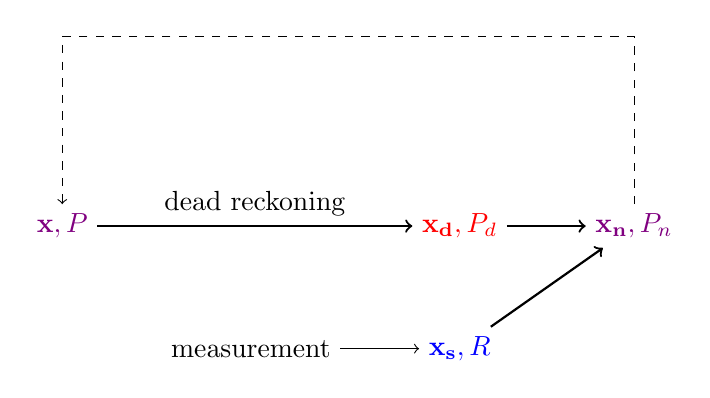
\begin{tikzpicture}
      \node[](before){\color{purple}$\mathbf{x},P$\cbla};
      \node[right = 4cm of before](dead){\color{red}$\mathbf{x_d},P_d$\cbla};
      \node[below = 1cm of dead](sensor){\color{blue}$\mathbf{x_s},R$\cbla};
      \node[right = 1cm of dead](new){\color{purple}$\mathbf{x_n},P_n$\cbla};
      \node[left  = 1cm of sensor](measure){measurement};
      \node[above = 2cm of new](anew){};
      \node[above = 2cm of before](abefore){};
      \draw[thick,->] (before)->node[above]{dead reckoning} (dead);
      \draw[thick,->] (dead)->(new);
      \draw[thick,->] (sensor)->(new);
      \draw[dashed,->] (new) -- (anew.center) -- (abefore.center) -> (before);
      \draw[thin,->] (measure) -> (sensor);
    \end{tikzpicture}
  \end{center}
\end{frame}



\begin{frame}{The Kalman filter and the brain}
  \begin{center}
    \includegraphics[width=7cm]{boxing1.png}
  \end{center}
\end{frame}


\begin{frame}{The Kalman filter and the brain}
  \begin{center}
    \includegraphics[width=7cm]{boxing2.png}
  \end{center}
\end{frame}


\begin{frame}{The Kalman filter and the brain}
  \begin{center}
    \includegraphics[width=7cm]{boxing3.png}
  \end{center}
\end{frame}


\begin{frame}{The Kalman filter and the brain}
  \begin{center}
    \includegraphics[width=7cm]{boxing4.png}
  \end{center}
\end{frame}

\end{document}
